
\documentclass[11pt,letterpaper,oneside]{article}
\usepackage[top=1.2in,left=1.3in,right=1.3in,bottom=1.2in]{geometry}
\usepackage{fancyvrb}
\usepackage{colortbl}
\usepackage{graphicx}

\title{Summary for Arum Development}
\author{Dejun Qian, Deron Jensen, Sisinty Sasmita Patra,  \\Department of Computer Science\\Portland State University\\Portland, OR\\dejun@pdx.edu}

\begin{document}
\maketitle

\begin{abstract}
This report summaries what have been done to extend the functionality of Arum.
\end{abstract}

% 1.  What you have contributed Arum/Tiptop.
% 2.  What challenges you faced or lessons learned.
% 3.  What you plan to complete before project is due.
% 4.  What future work can be done by another group.
\section{Introduction}
Arum is a light-weight performance measuring tool for applications, system and environment. In this project, we focus on extending Arum to profile applications on binary level. We use Dyninst to inject binary code into the application binary. We extend Arum in the following way:
\newline
\textbf{Build and Make existing code}
\begin{enumerate}
\item Reorganized code into /src /test /tools with docs and makefiles.  Tests are now merged into test directories and linked to ARUM libraries.
\item Added Makefile and instructions for Hardware counter kernel module.
\item Added usable error messages and exceptions for unsupported hardware (IA32).
\item Added accurate "usage" message to output.
\item Added environment variable for HwCtr module configuration and '-r' flag to allow ARUM to run on unsupported hardware, or outside of the "make" area.
\end{enumerate}
\textbf{Dynamic Instrumentation}
\begin{enumerate}
\item Build Dyninst library and integrate it into Arum.
\item List all the functions in the application along with the begining and end address of the code of each function.
\item Write the code to be injected into the application binary. The code will get the user time, system time and watch time at the executing time.
\item Inject the code into the begining and end of each function in the application.
\item Designed a machenism to pass the collected information from the application to Arum.
\item Generate the profiling report.
\item Designed a program to consume both measurable user time and measurable system time for testing purpose.
\end{enumerate}
\textbf{Testing}
\begin{enumerate}
\item Test ARUM command line options and existing functionality.
\item Test a function call.
\item Test a loop and recursive function call.
\end{enumerate}

\section{Methodology}
For ARUM, we looked at gprof style of output and Dyninst for dynamic instrumentation.  First, we needed to organize the ARUM code into a solid make and build exisiting tests with the ARUM code (not copies of the code).   Additionally we needed test cases for the new functionality, and a driver to test the programs.

The pseudo-code for the dynamic instrumentation is as follows:
\begin{Verbatim}[frame=single]
line 1: prepare the code for injecting
line 2: list all functions
line 3: for each function
line 4:   insert the code to the begining
line 5:   insert the code to the end
line 6:
line 7: fork and exec the revised binary
line 8: send the result to Arum
line 9: 
line 10: generate the report
\end{Verbatim}

The task of profile the application in binary mode is not trivial. We encountered the following challenges:
\begin{enumerate}
\item ARUM source code was duplicated and in several dispserse directories.  
\item Did not compile on IA32 (and other architectures).
\item HwCtr Module does not work as described in example (Don't know where the code is?)
\item Dyninst has several requirements to install and get working.
\item Can't use createProcess function. As a result, we can't inject the code into a running process. This problem is solved by rewriting the application binary before running the application.
\item Create customized structure when invoking times function to get the timestamps.
\item How to communicate with Arum as easy as possible.
\item Handle recursive function calls.
\end{enumerate}

For the purpose of profiling the application in binary image, we have collected enough information for further process. Based on these information, we can
\begin{enumerate}
\item recover the executing sequence of each function, when it begins and when it finishs.
\item give how many time does each function run
\item give how long does each function instance take to run in user time, system time and watch time.
\item give the average time each function takes to run.
\item give the calling hierarchy of the functions in the application.
\end{enumerate}
These task can be done by project 2. Using a good visualization technique will help Arum to present these information in a user friendly way.
\newline
To test this feature, we designed a test program which use noticable use time and system time. The functions implemented in the test program is listed in Fig \ref{fig:fake} - Fig \ref{fig:main}. In fig \ref{fig:fake}, we implement a function which will never be called in the program. Fig \ref{fig:foo} implement a funtion which spend competable time in user mode and kernel mode. Fig \ref{fig:recursive} is used to test recurseve functions. Fig \ref{fig:main} is the main function of the program.

\begin{figure}
\begin{center}
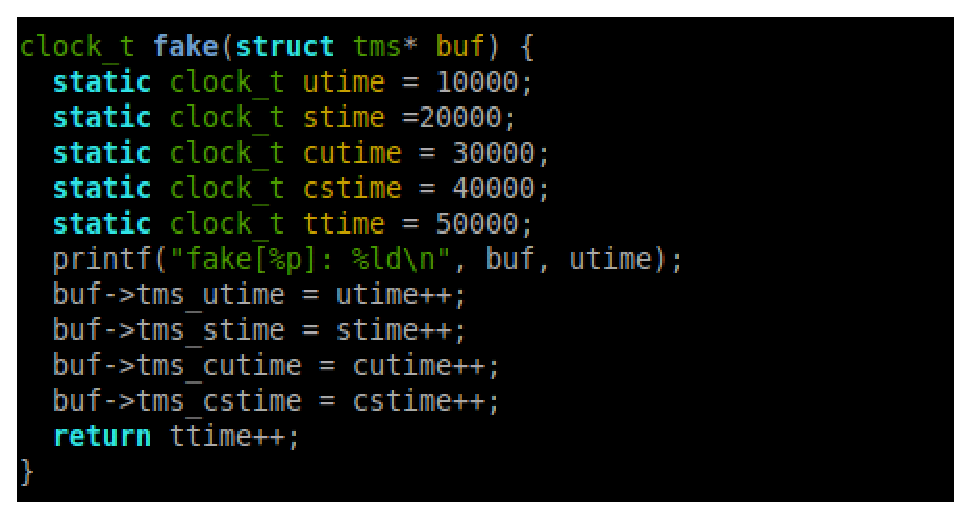
\includegraphics[width=0.9\textwidth]{fig4.eps}
\caption{fake function}
\label{fig:fake}
\end{center}
\end{figure}
\begin{figure}
\begin{center}
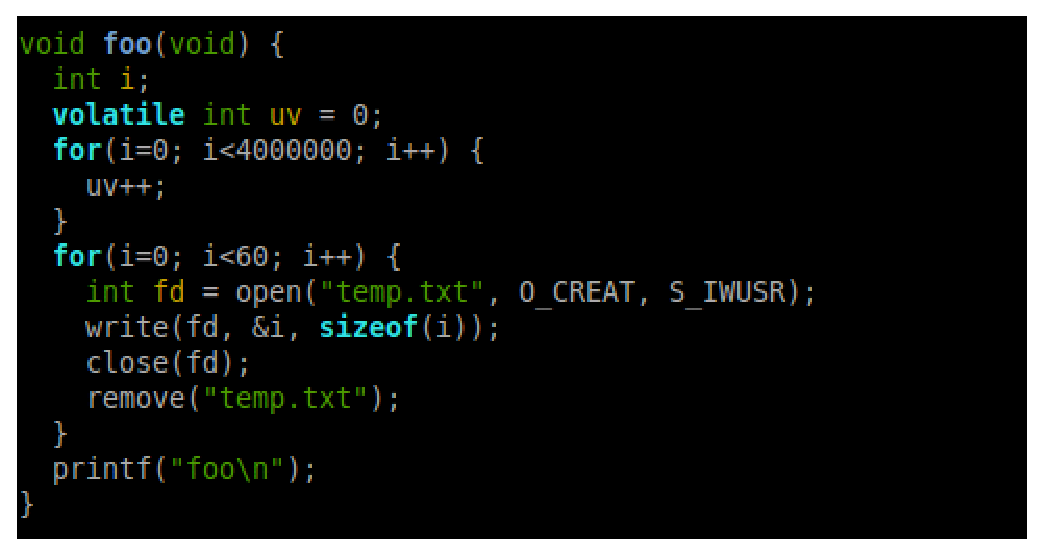
\includegraphics[width=0.9\textwidth]{fig5.eps}
\caption{foo function}
\label{fig:foo}
\end{center}
\end{figure}
\begin{figure}
\begin{center}
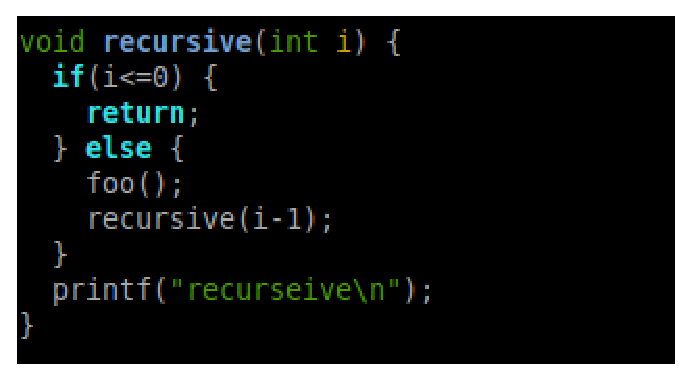
\includegraphics[width=0.6\textwidth]{fig6.eps}
\caption{recursive function}
\label{fig:recursive}
\end{center}
\end{figure}
\begin{figure}
\begin{center}
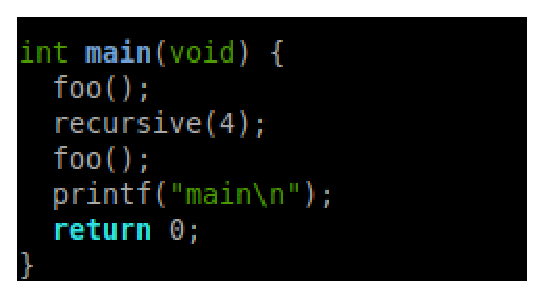
\includegraphics[width=0.5\textwidth]{fig7.eps}
\caption{main function}
\label{fig:main}
\end{center}
\end{figure}

\section{Results}
The result for the experiment is shown in fig \ref{fig:orig} - fig \ref{fig:trace}. Fig \ref{fig:orig} shows the result of the original version of Arum we get from the project assignment. From this point, we only get the user time and system time of the whole program. There is no value to have this information to improve the performance of the program, as it didn't give us where does the program need to be improved. Fig \ref{fig:list} is the result of the function list of the program output by the new version of Arum which is extended by this project. The is the first step of our implementation. This list can give us a general idea about the size of the program. The more functions the program has, the more complex the program is. Fig \ref{fig:trace} shows the execution trace of the program. The information includes the beginning time and end time of each function of both user time and system time as well as watch time. With these information, we can figure out which function is called more and need more attension.
\begin{figure}
\begin{center}
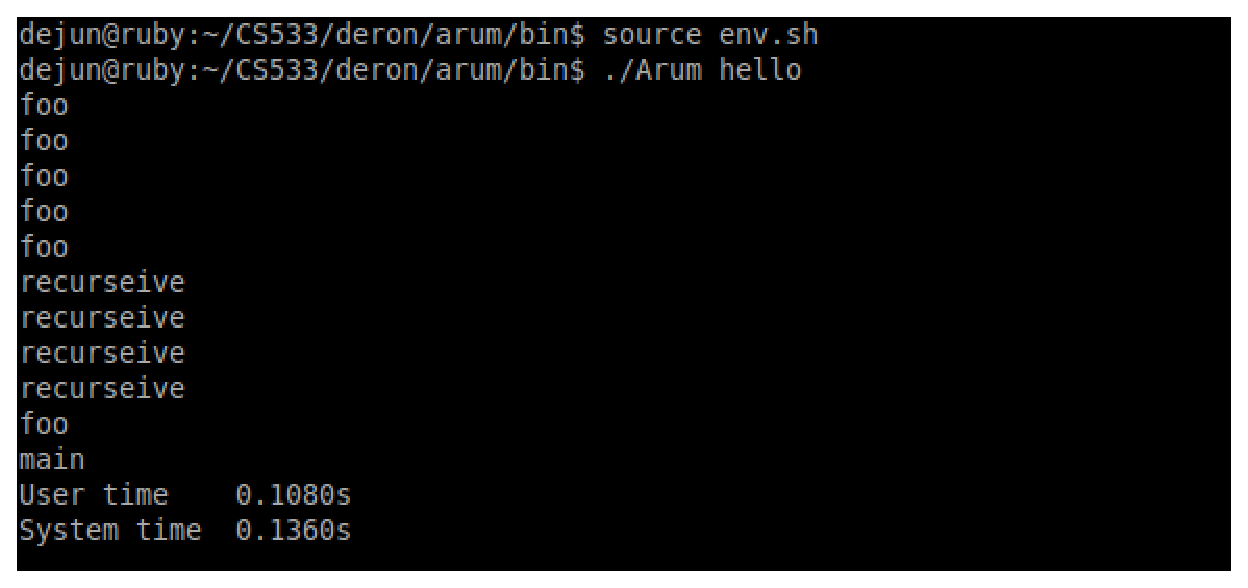
\includegraphics[width=6in]{fig1.eps}
\caption{output from the original}
\label{fig:orig}
\end{center}
\end{figure}
\begin{figure}
\begin{center}
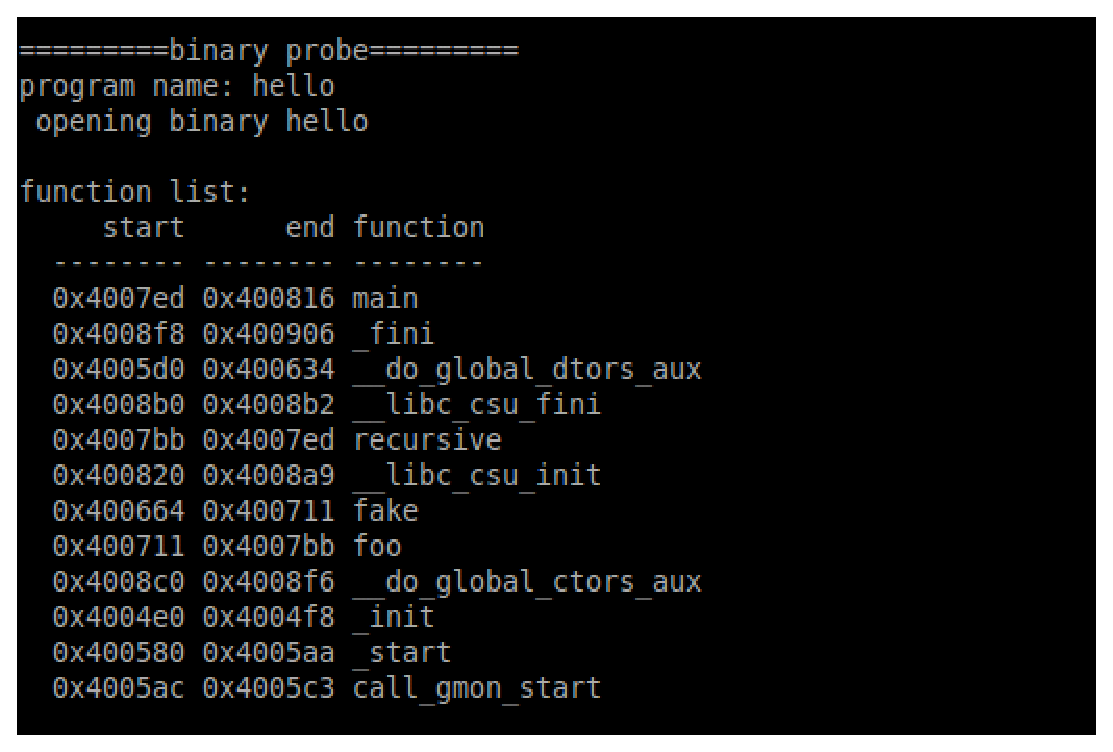
\includegraphics[width=6in]{fig2.eps}
\caption{function list}
\label{fig:list}
\end{center}
\end{figure}
\begin{figure}
\begin{center}
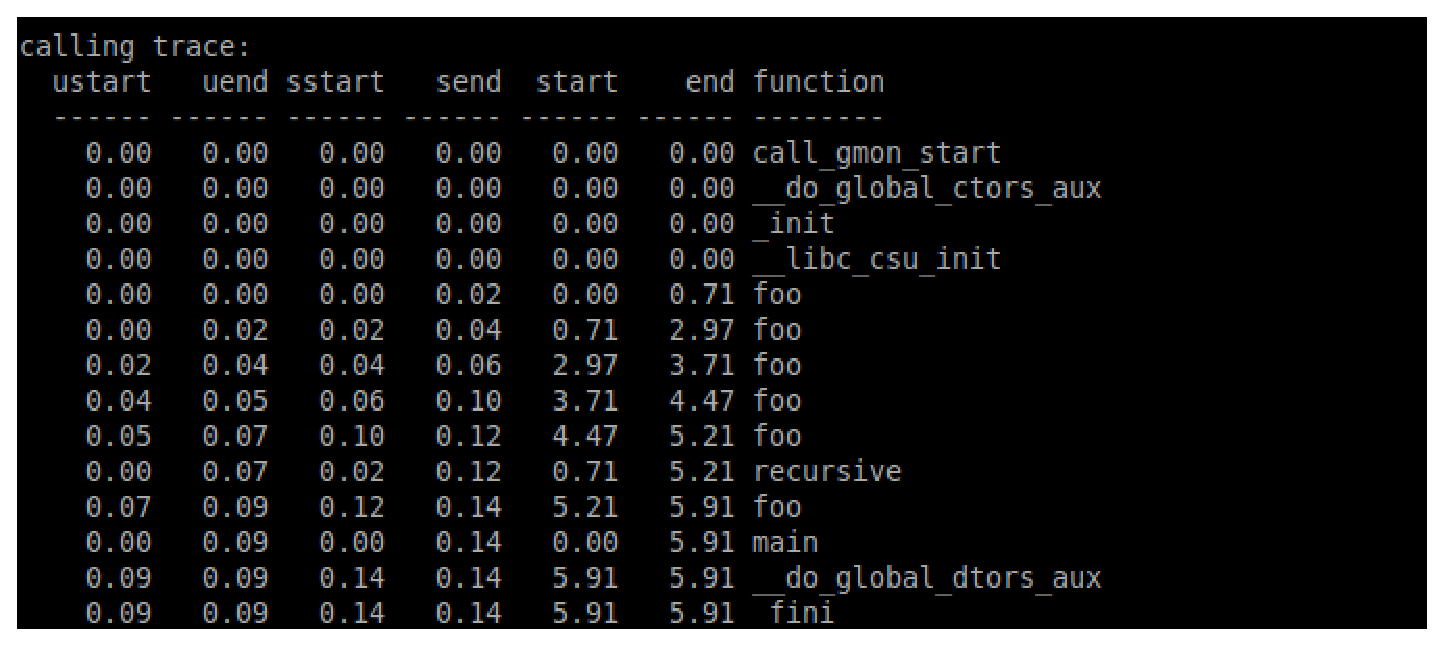
\includegraphics[width=6in]{fig3.eps}
\caption{execution trace}
\label{fig:trace}
\end{center}
\end{figure}

\section{Conclusions and Future Work}
There is still a great deal of opportunity to improve ARUM.   One of the future goals should be to allow ARUM to run on other hardware.  The kernel module currently only supports a single architecture (Intel-15-6).  Adding the Dyninst modules to the build is extremely difficult.  Dyninst requires much work to install on various architectures and platforms.   Currently the Dyninst is compiled and commited with the project.  It should be added as a separate module outside of the project.  Additionally the ARUM build should link with the location of the Dyninst.
\newline
The current instrumentation works, but needs to do some formatting of the output.  The data is available, but there may be other ways to present the information to the user of the program.
\newline
There are several tests that still need to be implemented to fully test all the functionality:
\begin{enumerate}
\item Planning to do tests for the command line option flags which give information of other metrics as well. 
\item Planning to come up with a test program that can be used as benchmark application for testing Arum functionalities with the ability to test features of Arum that include command line options, profiling for a single function, number of times the function is called and update test scripts once the	testing is automated.
\item Plan to use Arum as well as a widely-used profiling tool like gprof on the benchmark test application to compare and measure the efficiency,	overheads or improvements that can be done on Arum. 
\end{enumerate}

\section{References}
\begin{thebibliography}{9}
\bibitem{buck}
Buck, B., Hollingsworth, J. \emph{An API for Runtime Code Patching}. Computer Science Department: University of Maryland. 
\bibitem{knapp}
Knapp, R. L., Pase, D. M., Karavanic, K. L. \emph{ARUM: Application Resource Usage Monitor}.  Computer Science Department:  Portland State University.
\end{thebibliography}
\end{document}
